\chapter{PCM Module Implementation}\label{chap:module}
This chapter will focus on the implementation of the PCM module within the GVSoC framework.
We will start by introducing the architecture of the module and the data structures used to store the crossbar values.
Then we will analyse the MVM algorithm and how we can optimise it to achieve better performance.
The first step before starting the implementation is to define the constraints of the architecture and the software running the simulator.

\section{Architecture Constraints}\label{sec:arch_const}
Before analysing the module itself, it is important to define some hardware constraints of the hardware running the simulator and software constraints of the simulator itself.

\subsection{Hardware Constraints}\label{sec:hw_const}
The hardware running the simulator spans various architectures and configurations, from low-power laptops to HPC nodes and high-power workstations.
This is a major concern when writing optimised code, especially when micro-optimisations are considered.
For this reason, the optimisation will be maintained at a high abstraction level, avoiding architecture-specific features and the adoption of hardware acceleration.

\subsection{Software Constraints}\label{sec:sw_const}
The GVSoC framework is a C++ based SoC event simulator. While it supports many architectures and configurations, the software is intentionally single‑threaded to preserve event‑accurate simulations.
Simulations involving multiple clusters on HPC nodes and high‑performance workstations reveal that the main bottlenecks are single‑thread performance and memory consumption. Therefore, the proposed optimisations will target both CPU efficiency and RAM usage.

\section{PCM Module Architecture}\label{sec:module_arch}
The PCM module architecture is shown in Figure \picref{fig:PCM-Module-Architecture} in the previous chapter.

To summarise, the module is characterised by a matrix of tiles. Each tile is a 3D array itself with surface $X \times Y$ and depth $K$, with $K$ being the number of layers of PCM cells stacked on top of each other. Each cell is able to hold $n$ bits as variable resistance.
The tiles are interfaced with a set of DACs connected to the rows and ADCs connected to the columns, enabling bidirectional conversion of input vectors from digital to analog and output vectors from analog to digital, respectively.
This is the basic architecture of the PCM module used in this implementation.

\section{Module Data-Structures}\label{sec:module_data}
Based on the architecture of our module, we notice the need for a large memory bank capable of accommodating all the values.
To add an abstraction layer, we can model only the layers and matrix sectors without major concern for the physical layer.
The key challenge lies in defining a data structure to store all the weights within the matrix. Dynamically allocated arrays appear to be the best option, as they allow for a fully configurable design.

Then, it is crucial to define a matrix-vector multiplication algorithm to test the effectiveness of the data structure.
\begin{equation}
Y_{s\cdot J + j}=\sum_{i=0}^{I-1}(\sum_{l\in L_s} M_{s,l,j,i}\cdot X_i)
\label{MVM_imp}
\end{equation}
Where:
\begin{conditions}
    s & sector index\\
    j & tile row index\\
    J & number of rows in the tile\\
    l & layer index\\
    i & column index\\
    L_s & layers used in the sector\\
    I & number of columns in the matrix\\
    M & matrix\\
    X & input vector\\
    Y & output vector
\end{conditions}
The above equation describes the MVM operation performed by the PCM module. It iterates over each enabled sector $s$ and for each row $j$ of the tile, computes the dot product between the input vector $X$ and the corresponding row of the matrix $M$ across all enabled layers $L_s$.
We use this naive implementation to perform initial benchmarks and determine the best data structure.

\subsection{Data-structure Optimisation}\label{sec:data_opt}
The first step is to define a general data structure that can be used to store the values of the PCM module.

\subsubsection{4D Array}\label{sec:4d_array}
An immediate solution is to use a 4-dimensional dynamically allocated array. This architecture allows for easy access to each cell using a standard n-dimensional matrix approach. However, it is not optimal due to significant performance issues.
Dynamically allocated multidimensional arrays can create cache locality problems, which may lead to more cache misses and slow down the algorithm. Additionally, there is considerable overhead associated with pointer allocations and deallocations during the lifespan of the model object.
Another critical concern for this use case is suboptimal memory usage. Each allocation may not be contiguous in memory, resulting in fragmentation and inefficient use of available memory. Furthermore, pointer dereferencing and pointer arithmetic can lead to inefficient memory access patterns, especially with large matrix dimensions.

\subsubsection{Flat Buffer}\label{sec:flat_buf}
A second, more optimized approach would be to use a "flat" n-dimensional array. This solution requires more advanced indexing calculations, leading to significantly fewer instructions for memory allocation and deallocation. Implementing this approach results in noticeable performance improvements. 
Analysis of a test program using Cachegrind (a Valgrind tool that simulates cache access) shows a marked decrease in cache misses and a reduction in memory reads. The decrease in cache misses is due to the sequential storage of data, which is read from memory in a similar sequential manner. The reduction in memory reads occurs because contiguous memory allocation eliminates the overhead of pointer dereferencing.
One of the main drawbacks of this method is the need to manually compute the index of each cell. However, using inline functions, macros, and strategies for register reuse can help reduce complexity and the number of instructions required.

\subsection{Differential Algorithm}\label{sec:diff_algo}
Before focusing on specific optimisations for the MVM algorithm, it is important to note that the PCM module is capable of using differential weights.
This means that each weight is represented by two PCM cells, one for the positive part and one for the negative part: the final weight is computed as the difference between the two cells.
This approach allows for maintaining high precision despite the inevitable drift caused by the module's physical characteristics.
To accommodate this feature, without changing the data structure or the MVM algorithm, it's possible to use two computation passes.
\begin{equation}
Y_{s\cdot J + j}=\sum_{i=0}^{I-1}(M_{s,h_l,j,i}-M_{s,l_l,j,i})\cdot X_i = \sum_{i=0}^{I-1}M_{s,h_l,j,i}\cdot X_i -\sum_{i=0}^{I-1}M_{s,l_l,j,i}\cdot X_i
\end{equation}
Where:
\begin{conditions}
    h_l & High Layer\\
    l_l & Low Layer\\
\end{conditions}
This approach, while doubling the number of operations required, allows us to maintain the same data structure and MVM algorithm.
This trade-off is acceptable because the differential approach is not commonly used and the optimisations for one of the two cases are mutually beneficial.

\section{MVM Algorithm}\label{sec:mvm_algo}
In this section, we analyse and improve the MVM algorithm performance.

\subsection{Standard Implementation}\label{sec:std_imp}
The standard algorithm to compute an MVM using this PCM module is already described in the previous section [\ref{MVM_imp}].
While some faster algorithms for sparse \cite{abboud_time_2023} and band matrix are described in the scientific literature, it is notable that, in this generalised case, the matrix does not adhere to any of those rules, and keeping track of the non-zero elements would require additional memory, which is not optimal for our use case.
For this reason the optimisations will target the standard algorithm by working on the code and structures.

Looking at the data structure, we notice two main points. 
First of all, the matrix is already divided into blocks (tiles) and sectors.
As suggested by some studies \cite{yajnaseni_survey_2015}, granularity is one of the keys for fast MVMs and MMs algorithms.
Secondly, our MVMs compute row by vector, rows that are stored sequentially in our flat buffer, meaning our data already follows cache-friendly and granularity rules.
This implementation already offers performance speed-ups while closely simulating the PCM module.

\section{Optimisations}\label{sec:optim}
While this step is not necessary in a simulation environment, it is crucial to run big simulations in a reasonable time, even on low-power devices, enabling wider accessibility and usability.

\subsection{Improved Cache-friendliness}\label{sec:cache_friendly}
From the analysis of the standard implementation [\ref{MVM_imp}], there is still some potential for improvement in the cache friendliness.
In particular, the way layers and sectors are handled can be aligned to improve cache-friendliness.
\begin{equation}
    Y_{s\cdot J + j}=\sum_{l\in L_s}(\sum_{i=0}^{I-1} M_{s,l,j,i}\cdot X_i)
    \label{MVM_op}
\end{equation}
Improving cache locality can be achieved by rearranging the layers to be processed in the outer loop. By fully computing one layer before moving on to the next, we can access data in a more sequential manner. This approach results in fewer cache misses and reduces the number of data reads. 
It is important to consider this design change when designing the data structure, particularly regarding how layers and sectors are loaded into memory.
\begin{figure}
    \centering
    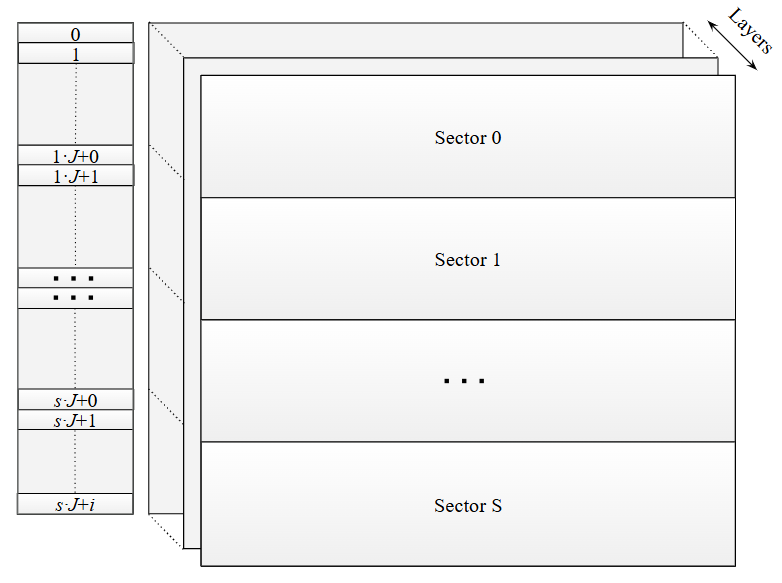
\includegraphics[width=0.5\textwidth]{Figures/pcm_cache_friendly.png}
    \caption{PCM matrix data-structure after cache-friendliness optimisation.}
    \label{fig:pcm_cache_friendly}
\end{figure}

\subsection{Register Reuse}\label{sec:reg_reuse}
Register reuse strategies are a great way to improve performance by reducing the number of memory accesses.
Specifically to this case, computing the sum of each row into a register without the need to store intermediate results in the output vector eliminates unnecessary memory writes and reads.
This approach leads to a significant reduction in memory accesses, with the only drawback that it is applicable only when the compiler is set to optimise the code.
Analysing the assembly code generated for each of the cases, it is immediately clear why.
In the non-optimised case the compiler store that same value on the stack and retrieves it at each iteration degrading the overall performances.\\

\lstdefinestyle{cleanasm}{
    language={[x86masm]Assembler},
    basicstyle=\tiny,
    keywordstyle=,
    commentstyle=,
    morekeywords={mov, push, lea, sub, add, cdqe},
    showstringspaces=false
}

\begin{table}[!ht]
\centering
\begin{minipage}[t]{.48\textwidth}
    \begin{lstlisting}[style=cleanasm,caption={Optimised Function Entry}]
        mov   r10, rdi
        push  r12
        lea   r9, [rcx+4]
        push  rbp
        mov   rbp, r8
        push  rbx
        mov   rbx, rdx
    \end{lstlisting}
\end{minipage}
\hfill
\begin{minipage}[t]{.48\textwidth}
    \begin{lstlisting}[style=cleanasm,caption={Un-Optimised Function Entry}]
        push  rbp
        mov   rbp, rsp
        push  rbx
        sub   rsp, 120
        mov   QWORD PTR [rbp-88], rdi
        mov   QWORD PTR [rbp-96], rsi
        mov   QWORD PTR [rbp-104], rdx
        mov   QWORD PTR [rbp-112], rcx
        mov   QWORD PTR [rbp-120], r8
    \end{lstlisting}
\end{minipage}

\vspace{0.5em} 

\begin{minipage}[t]{.48\textwidth}
    \begin{lstlisting}[style=cleanasm,caption={Optimised Variable Access}]
        movsx rdx, edi
        mov   r8, QWORD PTR [rbx+rdx*8]
    \end{lstlisting}
\end{minipage}
\hfill
\begin{minipage}[t]{.48\textwidth}
    \begin{lstlisting}[style=cleanasm,caption={Un-Optimised Variable Access}]
        mov   eax, DWORD PTR [rbp-24]
        cdqe
        lea   rdx, [0+rax*4]
        mov   rax, QWORD PTR [rbp-64]
        add   rax, rdx
        mov   eax, DWORD PTR [rax]
        mov   DWORD PTR [rbp-68], eax
    \end{lstlisting}
\end{minipage}

\caption{Comparison between optimised and un-optimised function setup and variable access code.}
\label{tab:asm_opt_comparison}
\end{table}
\subsection{Multithreading}\label{sec:multithread}
While cache-friendliness and register reuse are great ways to improve performance, multithreading is one of the best performance boosters in both MVMs and MMs.
\cite{yajnaseni_survey_2015,wyrzykowski_mathematical_2016,tang_multithreaded_2024,sulatycke_caching-efficient_1998}.
To both take advantage of multithreading, while minimising thread synchronisation and race conditions, which would slow down the algorithm, a modified implementation is proposed by moving some of the inner loops to different threads.
The loops in question are the sector loops.
This approach guarantees granularity and, because each result value is stored at a different vector index, there is no need to synchronise processes.
It is possible to increase the thread count beyond the number of sectors by splitting the row loop, but this requires proper synchronisation.
In this case, atomic operations are used; the overhead is minimal because the atomic operations are limited to the write operation of the output vector; however, the performance impact is still present.

While implementing multithreading is fairly straightforward, the problem lies in using the right number of threads.
Some studies suggest that the number of threads should be equal to the number of physical cores \cite{bhutani_exploring_2024}: Using more threads will lead to "over-threading" and, therefore, worsen the performance.
However, other studies suggest that the number of threads is, in small variation, independent of the number of physical cores and, especially in cases where synchronisation is not required, therefore suggesting that a different number of threads could be beneficial  \cite{cooper_how_2011}.
To explore this aspect, algorithm tests are proposed to determine the optimal number of threads for specific cases. The goal is to achieve results that are as general as possible for consumer hardware.

\section{Digital to Analog \& Analog to Digital Converters}\label{sec:mod_gvsoc}
\subsection{DAC}\label{sec:dac}
The Digital to Analog Converter (DAC) is a key component of the PCM module, responsible for converting digital input vectors into analog signals that can be applied to the rows of the PCM array.
However, there is no need to model the actual analog signal because the PCM model, being simulated on a digital platform, can directly work with digital values.
It is important to note that the DAC introduces latency that is annotated as part of the simulation.

\subsection{ADC}\label{sec:adc}
The Analog to Digital Converter (ADC) is another key component of the PCM module, responsible for converting the analog output signals from the columns of the PCM array back into digital values.
Similar to the DAC, there is no need to simulate the actual analog signal because the PCM model can directly work with digital values; however, the ADC will clip the output values to the maximum and minimum values representable by the number of bits used in the conversion.
To model this behaviour, the ADC model applies a  clipping function to the output values.
\begin{align}     
    n=output\;bit\;size\\
    ADC(y) = 
    \begin{cases}
    2^{n-1}-1 & \text{if } y > 2^{n-1}-1 \\
    -2^{n-1} & \text{if } y < -2^{n-1} \\
    y & \text{otherwise}
    \end{cases}
\end{align}
This function ensures that the output values are always within the valid range for the given output bit size.
Similar to the DAC, the ADC introduces latency that is annotated as part of the simulation.

\section{GVSoC Integration}\label{sec:gvsoc_int}
To integrate the PCM module into the GVSoC framework, we need to create a new peripheral class that represents the PCM.
This class will be responsible for handling the communication between the model and the rest of the system,
as well as managing the internal state of the PCM.
The PCM is implemented as a memory-mapped peripheral, allowing the processor to read and write data to the PCM using standard memory access instructions.
The module is connected to the system bus, allowing it to communicate with other peripherals and memory components in the system.
The bus interface has been implemented using the standard GVSoC wire.

The module has a defined mapping capable of exposing the memory space, read and write of the PCM cells, and the main AIMC unit, allowing the processor to store the input vector, trigger the MVM operation, write the input vector, and read the output vector.
All the operations expose the result immediately by queuing the result at the correct time; the only exception is the MVM operation, which, while taking place immediately, exposes the result after a defined latency once the event timer signals the module.
The PCM module also includes a set of configuration registers that allow the processor to configure the operation of the PCM module, such as the MVM dimensions, weights precision, and different MVM modes like signed and unsigned, or the previously described differential mode.
